% !TEX root = ../main.tex
% !TEX program = XeLaTeX
% !TEX encoding = UTF-8 Unicode

\date{2018년 3월 21일}

\begin{frontmatter}
\title{레즈기어}
\author{김민규}
\address{서울대학교}
\begin{abstract}
Haspelmath, Martin. (1993). A Grammar of Lezgian. Berlin, Boston: De Gruyter Mouton, 52--109.
\end{abstract}
\end{frontmatter}

%%%%%
\section*{발제 범위 분배}
\begin{table}[h]
\begin{center}
\def\arraystretch{1.5}
\begin{tabular}{>{\sffamily}ccccl}
\hline
	&\itshape 발제자	&\itshape 발제 범위
	&\itshape 페이지	&\itshape 내용\\
\hline
1	&양재영	&Ch. 1--4	&pp. 1--51			&서론, 화자, 분절음운단위, 음소배열론\\
2	&김민규	&Ch. 5--7	&pp. 52--109			&(형태)음운적 교체, 강세, 명사 형태론\\
3	&		&Ch. 8--9	&pp. 110--162		&형용사 형태론, 동사 굴절\\
4	&		&Ch. 10--12	&pp. 163--227		&동사 파생, 대명사, 부사 \& 후치사\\
5	&		&Ch. 14--15	&pp. 228--293		&수사 \& 불변화사, 명사구 \& 형용사구, 동사 결합가\\
6	&		&Ch. 16--19	&pp. 294--353		&절 통사론, 계사절, 등위접속, 관계절\\
7	&		&Ch. 20--21	&pp. 354--400		&보문절, 부사절\\
8	&		&Ch. 22--24	&pp. 401--441		&공지시, 의문문, 비교\\
\hline
\end{tabular}
\end{center}
\label{default}
\end{table}

\setcounter{section}{4}

\section{음운론적 교체}
\subsection{방출음 앞 방출음의 유기음화}
\begin{itemize}
\item CVC 구조의 단음절 명사들에서 V가 고모음일 때, 절대격 단수를 제외한 모든 형태에서는 강세가 어근 다음에 나타나게 되어 V가 축약되고 첫번째 C가 방출음에서 무성 파열음으로 교체되며, 음소배열론(4.3.1)에 따라 유기음이 된다.
\begin{figure}[H]
\centerline{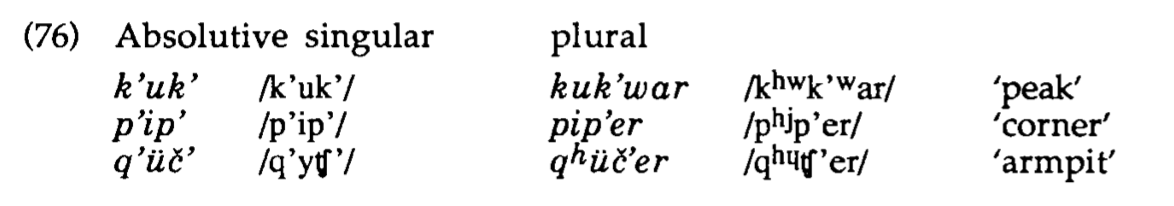
\includegraphics[width=.8\linewidth]{Lezgian/src/ex76.png}}
\end{figure}
\end{itemize}

\subsection{어말 무기음의 무성음화}
\begin{itemize}
\item 단음절 명사 어근말의 무성 무기음은 절대격 단수 형태에서 어말 환경에 놓이게 되어 유성음화한다. 
\item 단, /tʃ/, /ts/, /q/는 각각 /ʒ/, /z/, /ʁ/에 대응된다.
\begin{itemize}
\item 이는 역사적으로 */dʒ/, */dz/, */ɢ/ 였기 때문이다. (몇몇 방언들은 이를 보존한다.)
\end{itemize}
\begin{figure}[H]
\centerline{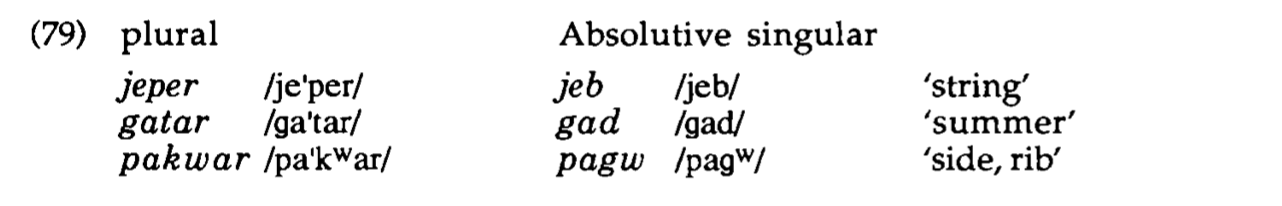
\includegraphics[width=.8\linewidth]{Lezgian/src/ex79.png}}
\end{figure}
\end{itemize}

\subsection{장애음 뒤 유기음의 무기음화}
\begin{itemize}
\item 단음절 명사들에서 V가 고모음이고, 어근두에 무기 장애음, 어근말에 유기 파열음이 있을 때, 어근말 자음은 절대격 단수를 제외한 모든 형태에서는 강세가 어근 다음에 나타나게 되어, V가 축약되고 어근말 자음은 음소배열론(4.3.2)에 따라 무기음화된다. 
\begin{figure}[H]
\centerline{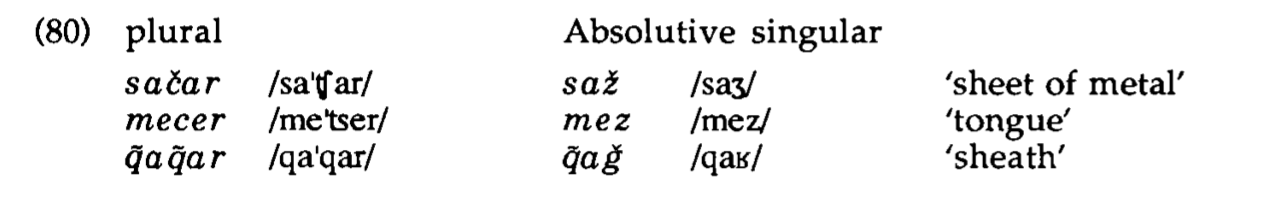
\includegraphics[width=.8\linewidth]{Lezgian/src/ex80.png}}
\end{figure}
\item 어근이 고모음이 아니어도 비강세 모음의 고모음화(5.11)이 먼저 일어나게 되면 같은 규칙이 적용된다.
\begin{figure}[H]
\centerline{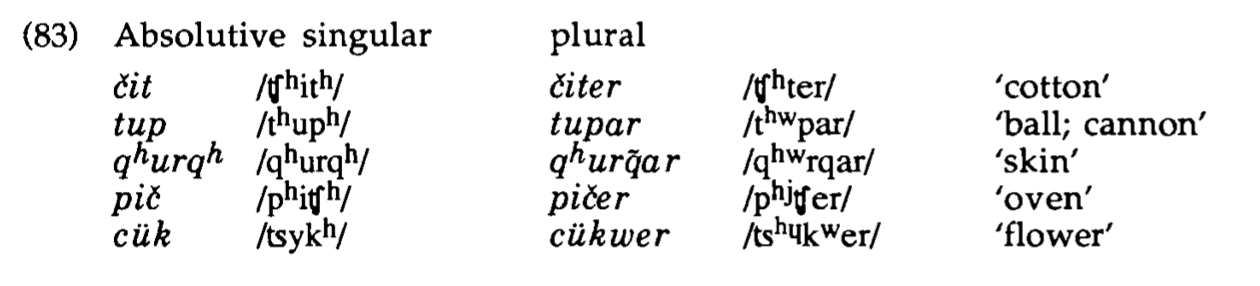
\includegraphics[width=.8\linewidth]{Lezgian/src/ex83.png}}
\end{figure}
\end{itemize}

\subsection{장애음 앞 무기음의 유기음화}
\begin{itemize}
\item 5.3와 같은 환경에서, 음소배열론에 따라 어근두 자음은 (반대로) 유기음화한다.
\begin{figure}[H]
\centerline{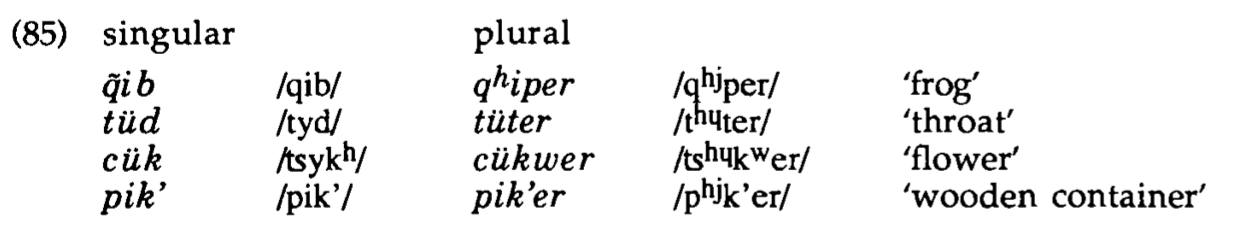
\includegraphics[width=.8\linewidth]{Lezgian/src/ex85.png}}
\end{figure}
\begin{itemize}
\item Uslar (1896)에서는 강세 앞 고모음 탈락이 일어나지 않아도 5.3 또는 5.4의 규칙이 적용된다는 패러독스가 발견된다. 이는 Uslar의 설명이 틀렸거나, 자음의 음소배열론이 꼭 자음이 완전히 인접해야하만 일어나는 것이 아니라서 그런 것일 수도 있다. 아마 Uslar 의 전사에서, 모음 탈락은 이미 일어났으나 남아있는 구개음화나 순음화를 표시하기 위해, \textbf{i, y, ü} 를 표기하였기 때문에 이런 혼동이 생긴 것으로 보인다.
\end{itemize}
\end{itemize}

\subsection{모음 조화 교체}
\begin{itemize}
\item 고유어의 접두사 및 강세를 가지는 접미사는 모음 조화에 의한 교체 현상이 존재한다. 
\begin{itemize}
\item 저모음을 가진 접사에서는 경구개 모음 조화(PVH)에 따라 /a/와 /e/가 교체된다. 
\item 분리내격(inelative) 접미사 \textbf{-äj/aj} 에서만 /a/와 /æ/가 교체된다. 
\item 고모음을 가진 접사에서는 경구개 모음 조화(PVH)와 원순 모음 조화(LVH)에 따라 /u/, /i/, /y/가 교체된다.
\item 이를 각각 \textbf{A} (/a/, /e/)와 \textbf{U} (/u/, /i/, /y/)로 나타낸다.
\begin{figure}[H]
\centerline{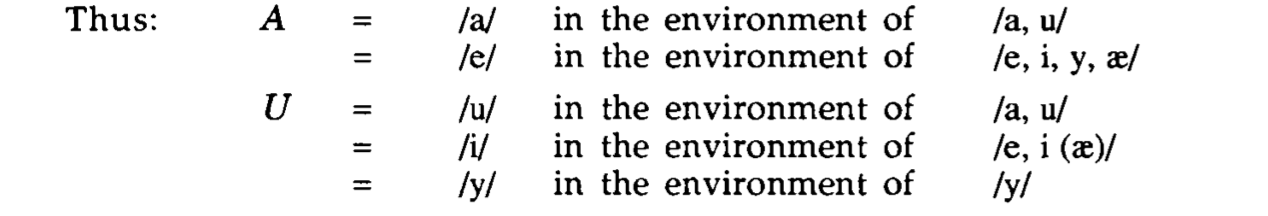
\includegraphics[width=.8\linewidth]{Lezgian/src/vh.png}}
\end{figure}
\item 예시: 복수 접미사 \textbf{-Ar}, 사격 접미사 \textbf{-rA}, 전동사(preverb) \textbf{A\~q-}, 부정 접두사 \textbf{tA-}, ...
\end{itemize}
\begin{figure}[H]
\centerline{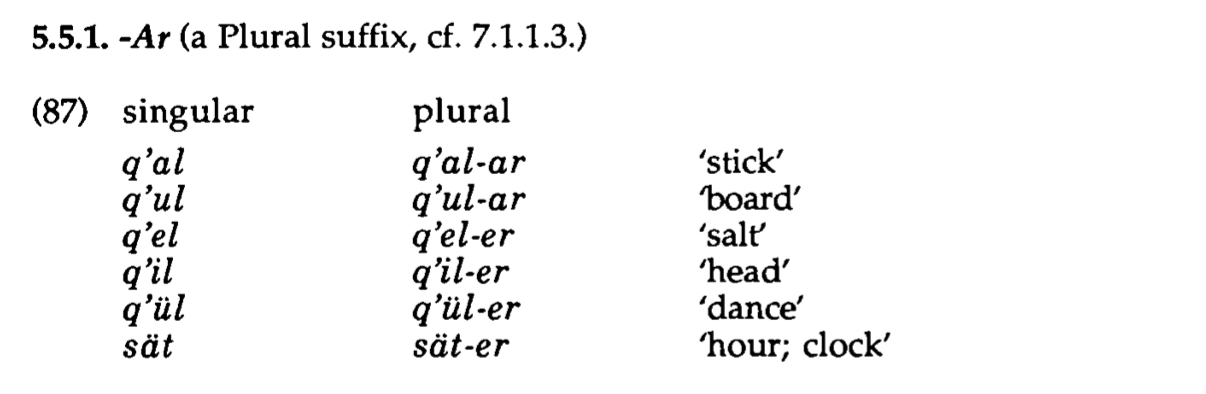
\includegraphics[width=.8\linewidth]{Lezgian/src/ex87.png}}
\end{figure}
\end{itemize}
 
\subsection{고모음 탈락}
\begin{itemize}
\item 강세 앞 고모음 탈락 현상에 따라 고모음을 가진 많은 단음절 명사들은 강세가 어근 뒤 음절로 옮겨갈 경우 모음이 탈락되고 구개음화 그리고/또는 순음화를 남긴다. (4.1.1 참조; 5.1, 5.3, 5.4에도 예시 존재)
\end{itemize}

\subsection{순음 장애음-모음 조화 교체}
\begin{itemize}
\item 고모음으로 시작하는 여러 접사가 /i/로 실현될 자리에서, 순음화된 자음에 인접할 경우 /y/로 실현된다.
\begin{figure}[H]
\centerline{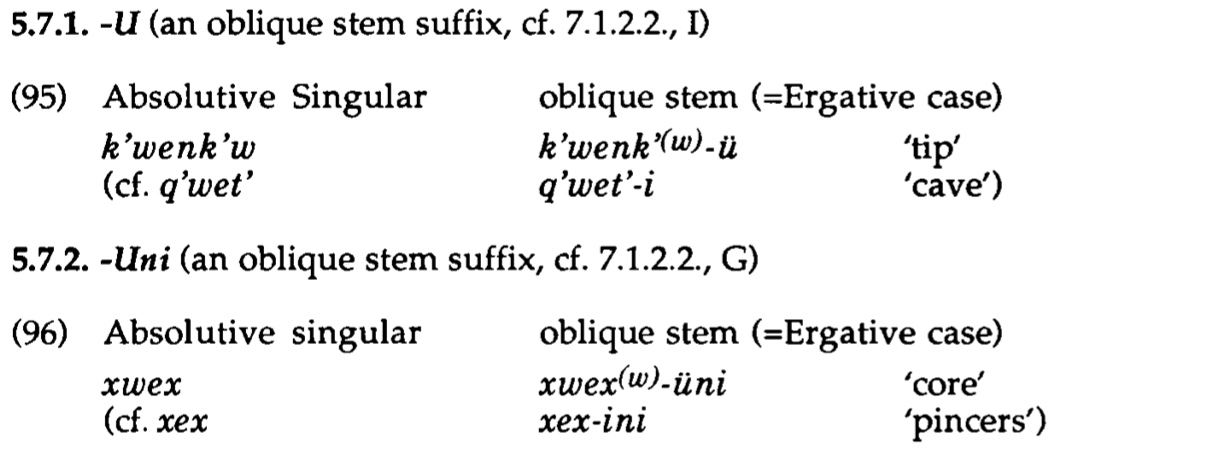
\includegraphics[width=.8\linewidth]{Lezgian/src/ex95.png}}
\end{figure}
\end{itemize}

\subsection{순음화의 음위 전환}
\begin{itemize}
\item 단어 마지막 음절의 모음이 원순음이 아니고, 어말 자음이 순음화된 자음일 경우, 실제 발음은 표기법과 다르게 순음화가 전위되어 나타날 수 있다.
\item 예: \textbf{tʼekw} [tʼʷek], \textbf{cegw} [tsʷeɡ], \textbf{tarkw}.[tʷarkʰ]
\item 심지어, 순음화된 자음이 음소적으로 존재하지 않는 자음에 대해서도 같은 규칙을 적용하는 화자도 있다. (예: \textbf{reğw} [rʷeʁ])
\item 종종 자음이 아니라 모을을 원순음화하는 경우도 존재한다.
\end{itemize}

\subsection{어말 방출음의 유기음화}
\begin{itemize}
\item 단음절 명사 어근말의 방출음은 절대격 단수 형태에서 어말 환경에 놓이게 되어 유기 파열음으로 변한다.
\begin{figure}[H]
\centerline{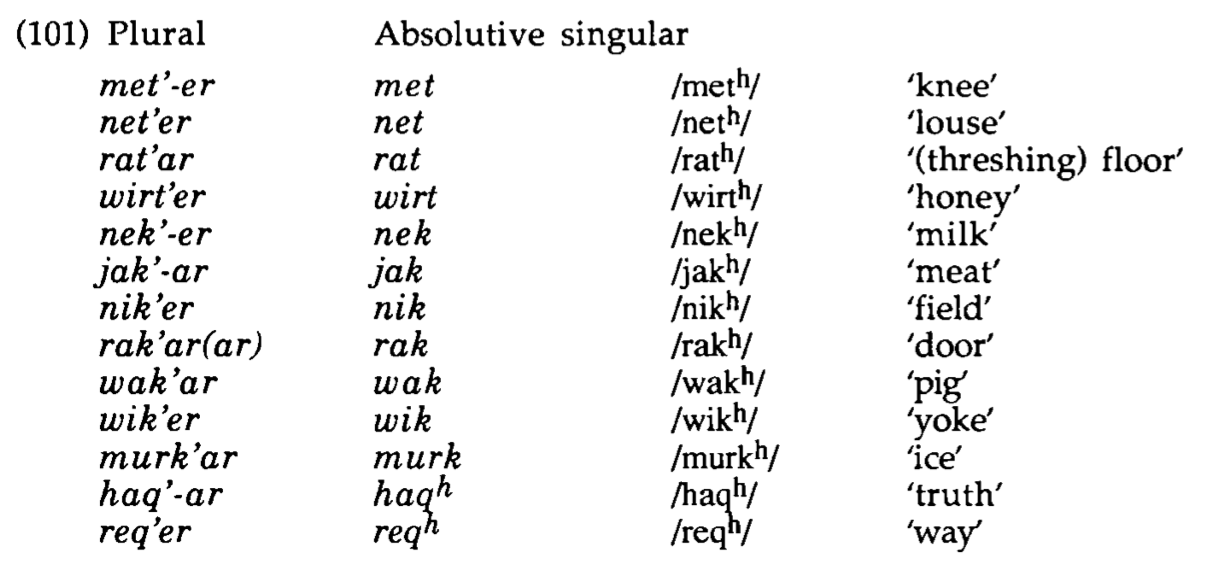
\includegraphics[width=.8\linewidth]{Lezgian/src/ex101.png}}
\end{figure}
\end{itemize}

\subsection{어말 방출음의 유성음화}
\begin{itemize}
\item 단음절 명사에서 어근두와 어근말의 자음이 모두 방출음일 경우, 어근말 방출은 절대격 단수 형태에서 어말 환경에 놓이게 되어 유성 파열음으로 변한다.
\begin{figure}[H]
\centerline{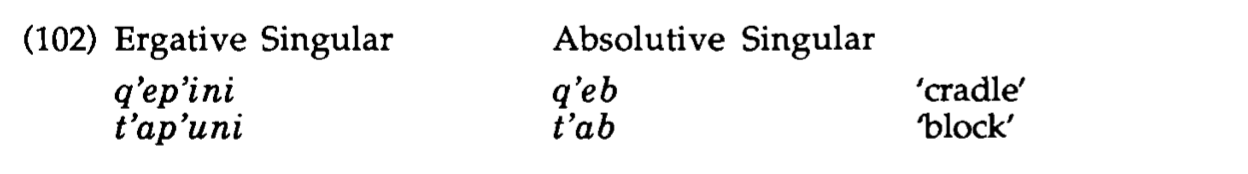
\includegraphics[width=.8\linewidth]{Lezgian/src/ex102.png}}
\end{figure}
\item 어근의 모음이 고모음일 경우, 절대격 단수를 제외한 형태에서는 방출음 앞 방출음의 유기음화(5.1) 현상이 일어나므로, 그 어떤 형태에서도 두 방출음이 모두 방출음으로 실현되지 않는다는 것을 알 수 있다.
\begin{figure}[H]
\centerline{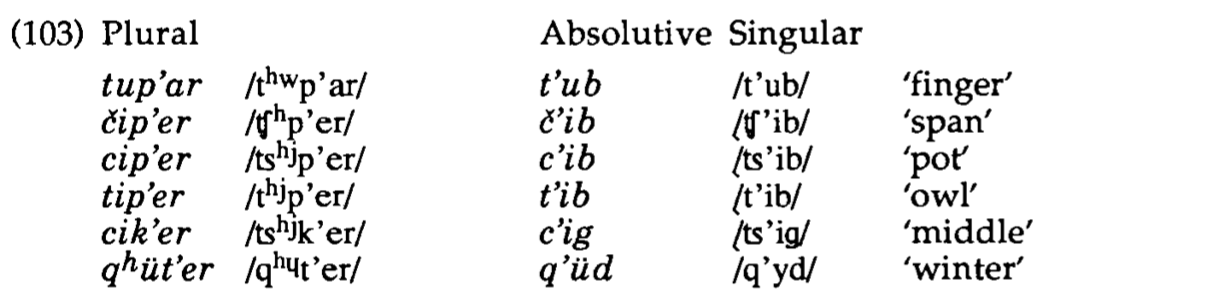
\includegraphics[width=.8\linewidth]{Lezgian/src/ex103.png}}
\end{figure}
\end{itemize}

\subsection{비강세 모음의 고모음화}
\begin{itemize}
\item CVC 구조의 단음절 명사들에서 V가 저모음일 때, 어근에 강세가 오지 않을 경우 고모음화한다. 조건에 따라서  강세 앞 고모음 탈락 규칙이 뒤이어 적용되기도 한다.
\begin{itemize}
\item /e/는 /i/로 교체되고, 순음화된 자음이 인접할 경우 /y/로 교체된다. 탈락되어 정서법상 사라지는 경우도 존재한다.
\begin{figure}[H]
\centerline{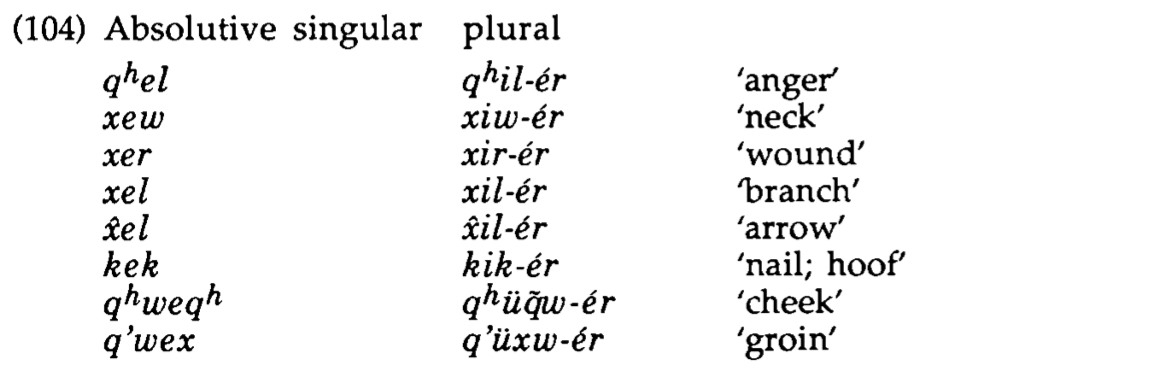
\includegraphics[width=.8\linewidth]{Lezgian/src/ex104.png}}
\end{figure}
\item /a/는 /i/로 교체되고, 순음화된 자음이 인접할 경우 /u/로 교체된다. /i/로 교체되는 경우는 무조건 탈락되며 현대 정서법 상에서 나타나지 않는다. 
\begin{figure}[H]
\centerline{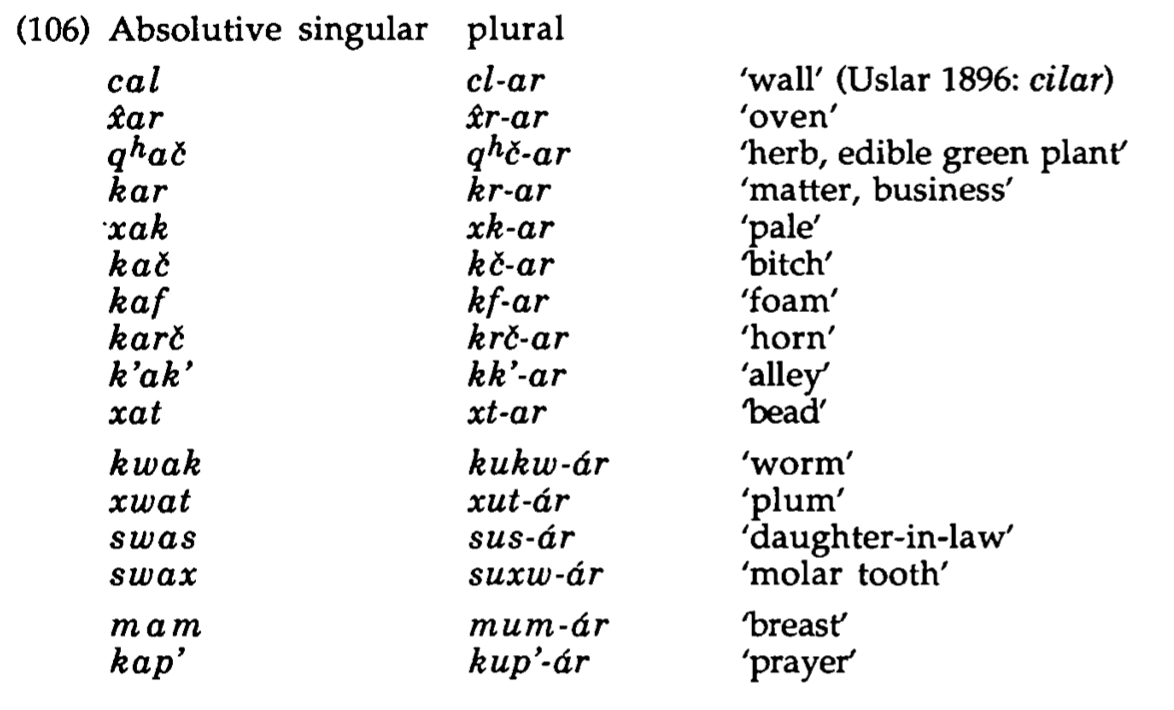
\includegraphics[width=.8\linewidth]{Lezgian/src/ex106.png}}
\end{figure}
\end{itemize}
\end{itemize}

\subsection{/ʁ/의 탈락}
\begin{itemize}
\item 적은 수의 동사들에게서 공통적으로 나타나는 어근인 \textbf{-äğun} 과 동사 \textbf{jağun} `hit'에서, 어근말 자음 /ʁ/는 모음이 후행하지 않을 경우 탈락되며 선행하는 모음이 보상적으로 장모음화한다. 다른 동사들은 이런 현상이 나타나지 않는다.
\begin{figure}[H]
\centerline{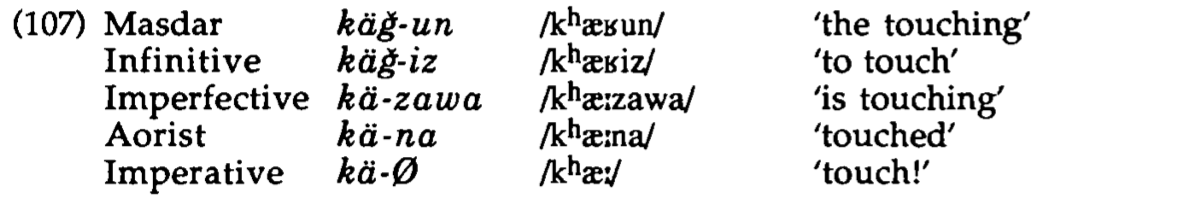
\includegraphics[width=.8\linewidth]{Lezgian/src/ex107.png}}
\end{figure}
\end{itemize}

\subsection{파찰음 동화}
\begin{itemize}
\item 사격 어간 접미사 \textbf{-ci} /-tsi/ (7.1.2.2 참조)는 \emph{부착되는 어근의 어두 자음}에 따라 \textbf{-cʼi}, \textbf{-či} /-tʃi/, \textbf{-čʼi}, \textbf{-ži} 등의 이형태가 존재한다.
\begin{figure}[H]
\centerline{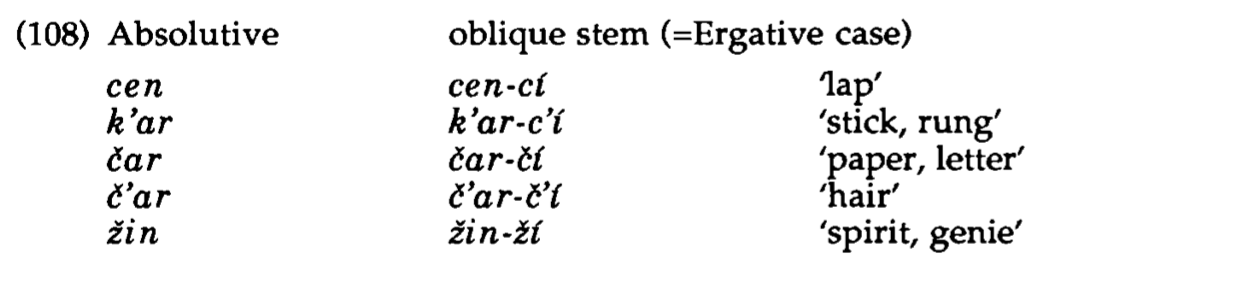
\includegraphics[width=.8\linewidth]{Lezgian/src/ex108.png}}
\end{figure}
\end{itemize}

\subsection{/r/의 이화 탈락}
\begin{itemize}
\item CVrC 구조의 단음절 명사에서, 사격 어간 접미사 \textbf{-rA} 가 부착되면, 어근의 \textbf{r}이 탈락된다. 음소배열론에 따라 CVrCrV 가 허락되지 않기 때문이다. 
\end{itemize}

\section{단어 강세}
\omission
%\subsection{어근의 강세}
%\subsection{접미사의 강세 성질}
%\subsection{모음 축약 후 레즈기어의 강세}

\section{명사 형태론}
\subsection{명사 굴절}
\subsubsection{복수형 형성}
\begin{itemize}
\item 복수형은 강세유인(stress-attrracting) 접미사 \textbf{-Ar} 또는 그 강세중립적 이형태인 \textbf{-ar}을 부착하여 형성된다. (예시는 본문 참조)
\begin{itemize}
\item 복수형 접미사의 기본형은 강세중립적 \textbf{-ar}이다. 거의 모든 다음절 명사에 부착. (예외 7.1.1.6)
\item 명사가 모음으로 끝날 경우에도 음절 수에 무관하게 \textbf{-ar}이 사용되며, 이 때 모음 충돌을 회피하기 위해 \textbf{j} 가 삽입된다.
\item 자음으로 끝나는 대부분의 단음절 명사는 \textbf{-Ar}가 사용된다. 많은 외래어에도 적용된다. 
\item 많은 단음절 외래어와 는 몇몇 단음절 고유어에도 \textbf{-ar}이 사용된다.
\item 후설 모음을 가진 몇몇 단음절 명사에는 \textbf{-ér}가 사용된다. Žirkov (1941:48)은 이러한 명사들의 대부분은 무성 연구개 또는 구개수음으로 시작한다는 점을 관찰했다.
\item 접미사 \textbf{-wal}을 이용하여 파생된 명사에는 \textbf{-er}가 사용된다.
\item 몇몇 단음절 명사(튀르크 차용어)는 \textbf{-lAr}이 사용된다. 이는 튀르크어족의 차용 접미사다.
\item 몇몇 명사는 \textbf{-Ar}의 중첩된 형태인 \textbf{-Arar}가 사용된다. 주로 쌍이나 집단을 나타내는 경우에 사용된다. 통시적으로, \textbf{-Ar}가 부착된 형태에 \textbf{-ar}가 한 번 더 부착된 것으로 추측된다.
\item 실질화(substantivizing) 접미사 중 단수형은 \textbf{-d}, 복수형은 \textbf{-bur}이다.
\item 표준 레즈기어에서는 러시아어 차용어의 몇몇 특수한 관행을 차용했다. 
\begin{itemize}
\item \textbf{-CR} (\textbf{R}=sonorant) 로 끝나는 러시아어 명사는 \textbf{-ajar/ijar}가 사용된다.
\item \textbf{-ie}, \textbf{oe}, \textbf{ee} 로 끝나는 러시아어 명사는 \textbf{-ijar}가 사용된다.
\item \textbf{-ja} 로 끝나는 러시아어 명사는 \textbf{-(ja)r}가 사용된다.
\end{itemize}
\end{itemize}
\item 복수형 접미사에 강세가 없을 경우, 모음으로 시작하는 사격 어간 접미사가 부착되면 모음 축약이 일어난다. (단, \textbf{-er}는 예외적으로 축약이 일어나지 않는다.)
\end{itemize}

\subsubsection{격 형성}
\begin{itemize}
\item 레즈기어에는 18개의 격이 있다.
\begin{itemize}
\item 4개의 문법적 격 (절대격, 능격, 속격, 여격)
\item 14개의 처소격 -- 5가지 국지(재, 후, 하, 상, 내)마다 3가지 처소격(상황격, 분리격, 방향격). 단, 내방향격(In-Directive)는 존재하지 않는다.
\end{itemize}
\begin{table}[H]
\centerline{
\begin{tabular}{ll>{\bfseries}l>{\itshape}ll}
\hline
절대격	&Absolutive		&sew			&`the bear'				&곰을; 곰이\\
능격		&Ergative		&sew-re			&`the bear'				&곰이\\
속격		&Genitive		&sew-re-n		&`of the bear'			&곰의\\
여격		&Dative			&sew-re-z		&`to the bear'			&곰에게\\
\\
재상황격	&Adessive		&sew-re-w		&`at the bear'			&곰에\\
재분리격	&Adelative		&sew-re-w-aj		&`from the bear'			&곰으로부터\\
재방향격	&Addriective	&sew-re-w-di		&`toward the bear'		&곰으로\\
\\
후상황격	&Postessive		&sew-re-qʰ		&`behind the bear'		&곰 뒤에\\
후분리격	&Postelative	&sew-re-qʰ-aj	&`from behind the bear'	&곰 뒤로부터\\
후방향격	&Postdirective	&sew-re-qʰ-di	&`to behind the bear'	&곰 뒤로\\
\\
하상황격	&Subessive		&sew-re-k		&`under the bear'		&곰 아래에\\
하분리격	&Subelative		&sew-re-k-aj		&`from under the bear'	&곰 아래로부터\\
하방향격	&Subdirective	&sew-re-k-di		&`to under the bear'		&곰 아래로\\
\\
상상황격	&Superessive	&sew-re-l		&`on the bear'			&곰 위에\\
상분리격	&Superelative	&sew-re-l-aj		&`off the bear'			&곰 위로부터\\
상방향격	&Superdirective	&sew-re-ldi		&`onto the bear'			&곰 위로\\
\\
내상황격	&Inessive		&sew-re			&`in the bear'			&곰 안에\\
내분리격	&Inelative		&sew-räj		&`out of the bear'		&곰 안으로부터\\
\hline
\end{tabular}}
\end{table}
\item 속격과 여격은 사격 어간(=능격)에 각각 \textbf{-n}, \textbf{-z}를 부착하여 형성한다.
\item 재, 후, 하의 국지는 사격 어간에 각각 \textbf{-w}, \textbf{-qʰ}, \textbf{-k}를 부착하여 형성한다. 분리격, 방향격은 각각 \textbf{-aj}, \textbf{-di}를 부착하여 형성한다.
\item 사격 어간은 다음과 같은 10가지 접미사를 통해 형성된다: \textbf{-di, -a, -i, -u, -Adi, -rA, -Uni, -A, -U, -ci/cʼi/či/čʼi/ži} (예시는 본문 참조)
\begin{itemize}
\item 기본형은 \textbf{-di}이다. 다음절 명사는 대부분 \textbf{-di}가 사용된다.
\item 모음으로 끝나는 단음절 명사에도 \textbf{-di}가 사용된다.
\item 자음으로 끝나는 인명은 \textbf{-a}가 사용된다. 인명이 일반명사를 따왔을 경우에도 마찬가지이다.
\item 적은 수의 일반 명사에도 \textbf{-a}가 사용된다.
\item \textbf{-wal}로 끝나는 추상명사와 \textbf{-(u)n}로 끝나는 Masdars (동명사?) 형태는 \textbf{-i}가 사용된다.
\item 모든 복수형 명사에도 \textbf{-i}가 사용된다. 단, \textbf{-bur}로 끝나는 복수형 제외.
\item 파생 명사가 아님에도 불구하고 단수형에 \textbf{-i}가 사용되는 명사가 존재한다. 그들 중 일부는 \textbf{-(u)n} 또는 \textbf{-r} 로 끝나는데, 통시적으로 Masdars 형태가 어휘화되었거나 \textit{pluralia tantum} 형태에서 단수형으로 재분석되었을 가능성이 있다.
\item 단음절 명사 중 접미사 \textbf{-i}가 강세유인을 하는 경우가 있다. 보통, 불규칙 복수형 접미사 \textbf{-er}를 취하는 명사들이다.
\item \textbf{-bur}로 끝나는 복수형은 \textbf{-u}가 사용된다.
\item 강세유인 \textbf{-Adi}는 단음절 명사중 비분리적 물질명사에 사용된다.
\item 강세유인 \textbf{-rA}는 고유어 단음절 명사 중 동물에 사용된다. 사람과 물건도 종종 있다.
\item 그 외 \textbf{-Uni, -A, -U, -cí/cʼí/čí/čʼí/ží}는 모두 강세유인이지만 선택되는 의미적, 형태론적, 음운론적 규칙이 없는 듯 보인다. 개별적으로 외워야 한다.
\item \textbf{-Uni}는 불규칙 접미사 중 유일하게 생산적이며, 차용어에도 사용된다. 이형태 \textbf{-ini}가 사용되는 두 경우가 있다.
\item \textbf{-cí}는 \textbf{*-dí}에서 유래하였다.
\end{itemize}
\item 내(In)의 국지는 자음으로 결정되지 않고, 사격 어간의 마지막 모음을 저모음화하여 표시한다.
\begin{itemize}
\item 강세를 가진 \textbf{-ú, -\'ü, -í}은 각각 \textbf{-á, -é, -é}로 변한다.
\item 비강세 \textbf{-u, -a}는 \textbf{-a}로 변한다. (단, 추상 접사 \textbf{-wil}가 있을 때는 \textbf{-i}가 \textbf{-e}로 변한다.)
\item 마지막 모음이 이미 저모음이면, 내상황격은 사격 어간(능격)과 형태가 같다.
\item 만약, 내상황격이 \textbf{-e}로 끝나면 내분리격은 \textbf{-aj}와 합쳐져 \textbf{-äj}가 된다.
\end{itemize}
\item 상(Super)의 국지는 사격 어간에 \textbf{-l}이 바로 부착되지 않고, 마지막 모음이 저모음화 된 뒤에 부착된다. 즉, 내상황격에 부착된다고도 말할 수 있다.
\begin{itemize}
\item 상방향격은 완벽히 규칙적으로 상상황격에 \textbf{-di}를 부착하여 얻어지지만, 상분리격을 형성할 때에는 사격 어간의 접미사가 강세를 받을 때에만 저모음화한다는 불규칙성이 있다.
\end{itemize}
\item 속격의 축약형
\begin{itemize}
\item 사격 어간 접미사가 강세를 받지 않고, \textbf{-i}로 끝나면, 속격의 \textbf{-in}이 탈락될 수 있다. 
\item 주로, 소유자가 지시적이지 않을 때 속격의 축약형이 사용된다. 영어의 합성 명사에서 앞 단어에 해당된다고 할 수 있다.
\item Talibov (1985)는  속격 축약형의 실질화 복수형이 `X와 X 주의의 사람들'이라는 특수한 용법으로 사용한다고 서술한다. Talibov는 이를 ``한정 수 (또는 paucal)''라고 부른다.
\begin{figure}[H]
\centerline{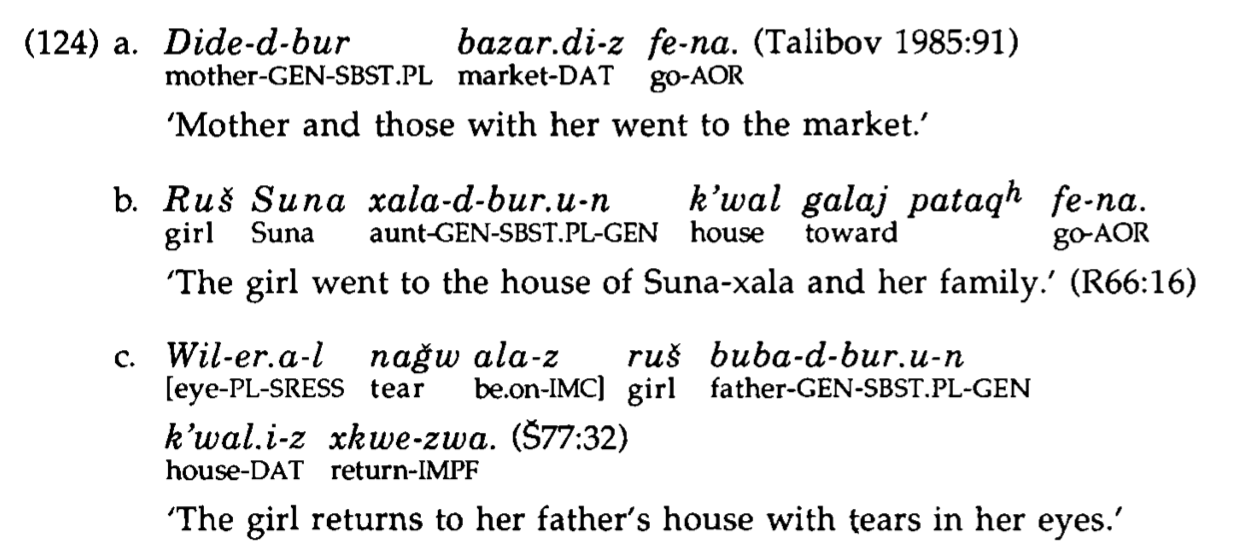
\includegraphics[width=.8\linewidth]{Lezgian/src/ex124.png}}
\end{figure}
\end{itemize}
\end{itemize}

\subsubsection{교체}
(5. 참조)

\subsubsection{불규칙}
\begin{itemize}
\item 다음은 불규칙 명사 굴절의 전체 목록이다.
\begin{figure}[H]
\centerline{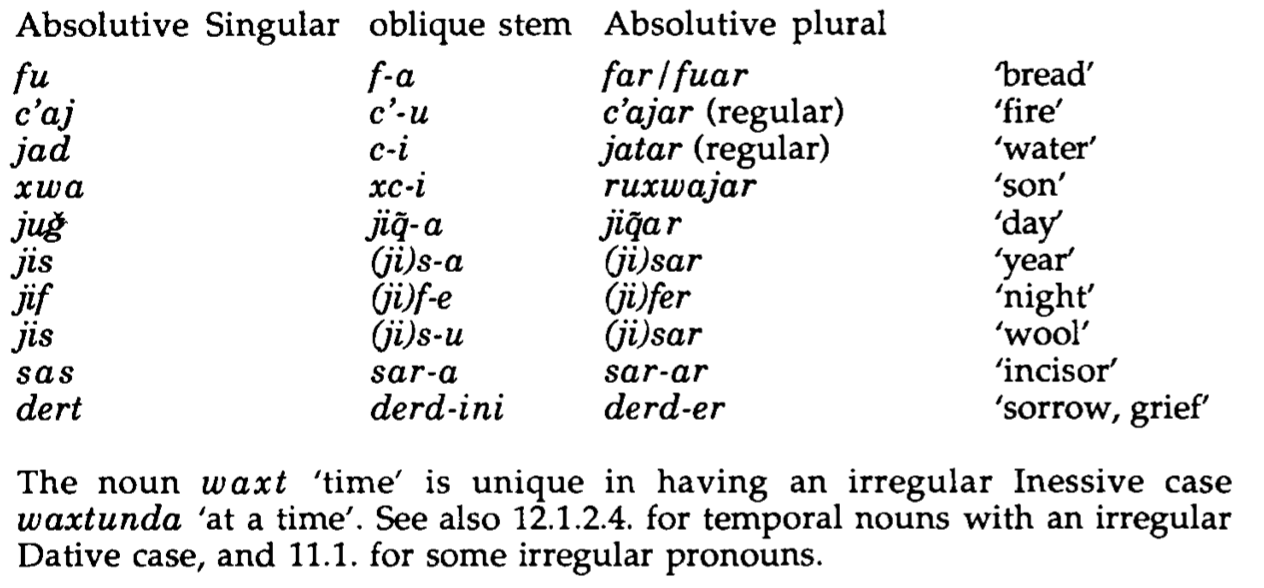
\includegraphics[width=.8\linewidth]{Lezgian/src/ex7-1-4.png}}
\end{figure}
\end{itemize}

\subsubsection{패러다임 예시}
\begin{itemize}
\item 다음은 명사 굴절 패러다임의 예시이다.
\begin{figure}[H]
\centerline{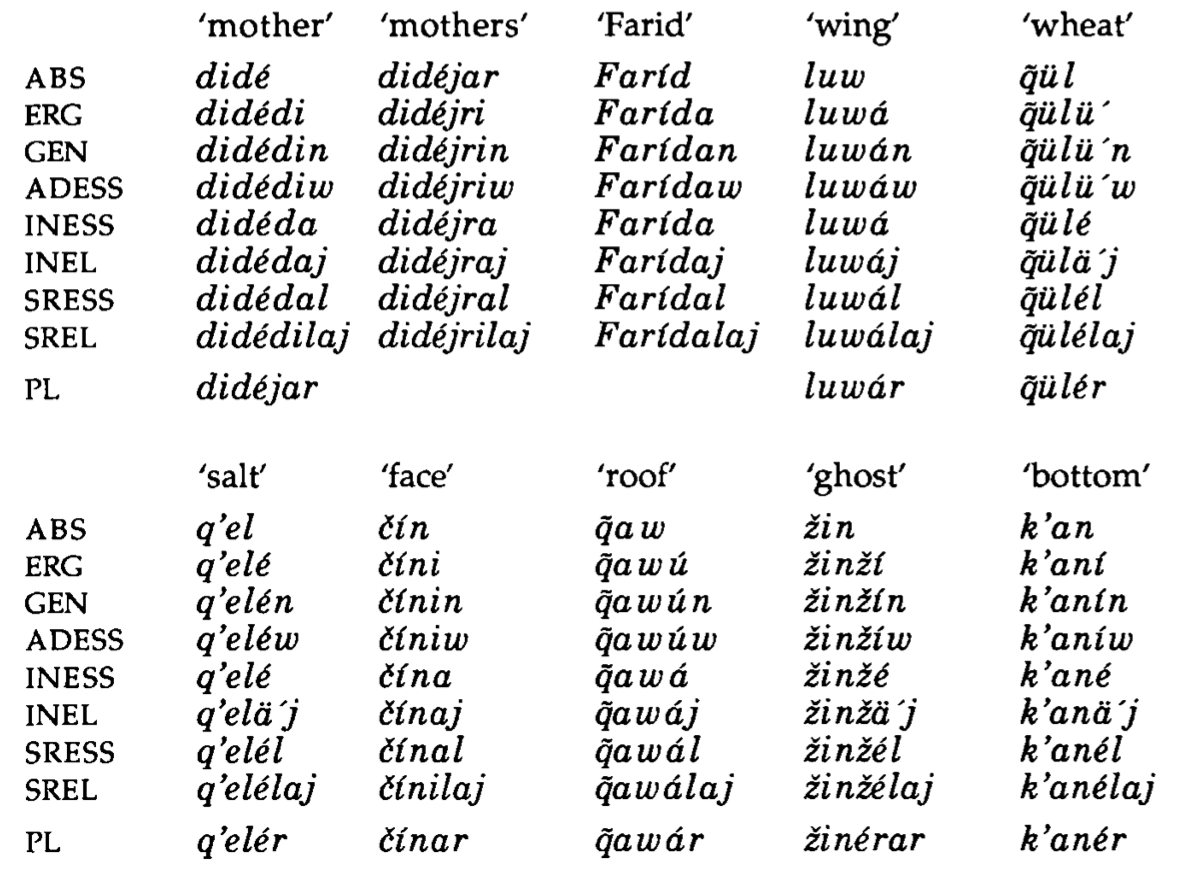
\includegraphics[width=.8\linewidth]{Lezgian/src/ex7-1-5.png}}
\end{figure}
\end{itemize}

\subsection{명사 굴절 카테고리의 기능}
\subsubsection{복수형의 기능}
\begin{itemize}
\item 복수형은 대상이 복수일 때 사용되며, 수사가 사용될 때에는 단수형이 사용된다.
\item 비가산 명사에 대해서도 복수형이 사용되며, 그 의미가 항상 직관적이지는 않다. 주로 많은 양을 의미한다.
\item 유일한 대상이나 추상적인 개념에 대해서도 사용되며, 성씨에 사용되어 가족을 나타내기도 한다.
\item \textit{pluralia tantum} 형태가 존재하여, 물질 또는 질병을 나타내기도 한다. 러시아에서  \textit{pluralia tantum} 형태인 것은 그대로 차용된다.\\
\NB \quad 이는 \textbf{-ar/er}로 끝나고 불규칙 사격 어간 접미사 \textbf{-i}를 취하는 몇몇 단수형 명사들과 혼동해서는 안된다. 진짜 \textit{pluralia tantum} 형태의 명사들은 복수 접미사를 추가적으로 부착할 수 없고, 형용사의 실질화 술어와 일치할 때 복수형으로서 일치한다.

\item \textit{pluralia tantum} 형태 중에서 뒤섞인 행동을 하는 경우도 존재한다. 여전히 복수 접미사를 부착할 수는 없지만, 양화사를 취하기도 하고, 단수형 실질화 술어와 일치하기도 한다.
\item 몇몇 레즈기 마을 이름은 \textit{pluralia tantum} 형태로 되어 있다.

\end{itemize}

\subsubsection{격들의 기능}
\paragraph{절대격}
\begin{itemize}
\item 레즈기어의 능격-절대격 체계는 표준적이다. 절대격은 자동사의 유일 논항 또는 타동사의 피동작주에 사용된다.
\item 명사 술어 구문의 명사구에서도 절대격이 사용된다.
\item 시간의 지속을 나타내는 몇몇 명사에 절대격이 사용되어 기간을 나타내기도 한다. 
\item 호격 명사구에도 사용된다.
\item 그 외에도, 부분 구(partitive phrase), 동격, 후치사 \textbf{patal}의 논항으로 사용된다.
\end{itemize}
\paragraph{능격}
\begin{itemize}
\item 능격 타동사의 동작주 논항에 사용된다.
\item \textbf{awun-}과 합성된 복합 동사의 유일 논항에도 사용된다. (15.4.2 참조)
\item 타동사의 동작주에는 유생성의 제약이 없다.
\item Talibov \& Gadžiev (1966)은 몇가지 도구로서의 기능을 제시하지만 현대에는 사용되지 않는 기능이다.
\end{itemize}
\paragraph{속격}
\begin{itemize}
\item 대부분의 언어와 비슷한 용도로 사용된다. 분리적, 비분리적 소유에 사용된다.
\item 부분-전체 관계, 동사 파생 명사에서의 A 또는 S 논항, 형용사 파생 명사에서의 S 논항
\item 성질, 재료, 각종 추상적 관계에 대해서도 사용된다.
\item 동격에는 사용되지 않는다.
\item 러시아어나 영어에 나타나는 관계 형용사를 비지시적인 속격으로 표현하기도 한다. (한국어와 비슷)
\item 레즈기어의 비지시적인 속격은 영어의 합성 명사에서 앞 단어와 비슷한 역할을 하기도 한다.
\item 명사에 부차적으로 나타나지 않는 용법으로는, 공간 표현 또는 시간 표현과 어울려 쓰여 공간적 또는 시간적 간격을 나타낼 때 사용된다.
\item 각종 후치사에 의해 지배된다.
\end{itemize}
\paragraph{여격}
\begin{itemize}
\item 수혜자, 경험자, 방향, 시간 등에 사용된다. 
\item 공간적 의미로 사용될 경우, 존재하지 않는 ``내방향격''을 대신한다.
\item 신체 부위와의 소유 관계에도 사용된다.
\item 적은 수의 경험 동사의 경험자와 많은 수의 경험 구조에서 경험자에 사용된다.
\item 소유 구문에서 소유자로 사용할 수 있다. 이 자리에 후상황격도 사용할 수 있다.
\item 시간을 나타낼 때에는 시간 상의 특정 지점을 표현한다.
\end{itemize}
\paragraph{처소격}
\omission

\subsection{명사 파생}
레즈기어의 명사 파생 패턴은 풍부하지 않다. 몇 개의 접미사가 약간의 생산성을 보이고, 명사 합성 또한 제한적이다.
\subsubsection{파생 접미사}
\begin{itemize}
\item 아래 8개의 접미사 중 3개만 고유어이고, 차용어 접미사는 완전히 생산적이지 않다.
\begin{figure}[H]
\centerline{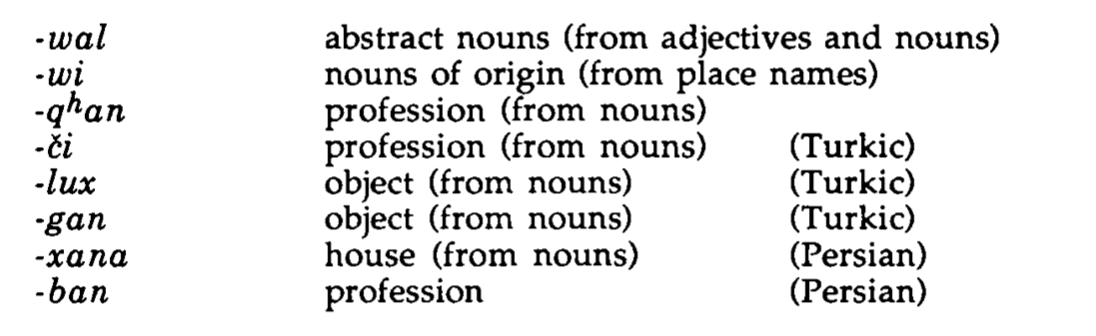
\includegraphics[width=.8\linewidth]{Lezgian/src/ex7-3-1.png}}
\end{figure}
\end{itemize}
\paragraph{-wal}
\begin{itemize}
\item \textbf{-wal}은 추상 명사를 파생시키는 매우 생산적인 접미사다.
\item 질적 형용사, 명사, 몇몇 부사로부터 파생이 가능하다.
\item \textbf{X-wal awun} (lit. `do X-hood'), \textbf{X-wile kʼwalaxun} (lit. `work X-hood')에서는 `as an X' 라는 의미의 직업 또는 기능의 역할을 한다.
\item 동사의 participial 형태에 부착되기도 한다. 
\item 목적, 태도를 의미하는 부동사(副動詞, converb) \textbf{-wal}와 동음이의어다. 어원론적으로 동일할 수도 있다.
\end{itemize}
\paragraph{-wi}
\begin{itemize}
\item \textbf{-wi}은 장소로부터 기원한 대상을 파생시키는 생산적인 접미사다. (\textbf{axcehwi} `person from Axceh') 
\item 사격 어간에서는 \textbf{-žuwa}로 교체된다.
\item 일반명사에서 파생된 형태도 존재한다. (\textbf{xürünwi} `villager', \textbf{dağwi} `mountain dweller')
\end{itemize}
\paragraph{-qʰan}
\begin{itemize}
\item \textbf{-qʰan}은 행위자를 파생시키는 접미사로, 생산적으로 보이지 않는다.
\end{itemize}
\paragraph{-či}
\begin{itemize}
\item \textbf{-či}는 튀르크 차용 접미사로, 행위자를 파생시키는 접미사이다.
\item 튀르크 또는 아랍 기원 어간에 부착된다.
\end{itemize}
\paragraph{-lux}
\begin{itemize}
\item \textbf{-lux}는 튀르크 차용 접미사로, 명사와 관련된 장소를 파생시키는 접미사다.
\end{itemize}
\paragraph{-gan}
\begin{itemize}
\item \textbf{-gan}는 튀르크 차용 접미사로, 명사가 담긴 용기를 파생시키는 접미사다.
\end{itemize}
\paragraph{-xana}
\begin{itemize}
\item \textbf{-xana}는 페르시아어 차용 접미사로, 명사와 관련된 집(건물)을 파생시키는 접미사다.
\end{itemize}
\paragraph{-ban}
\begin{itemize}
\item \textbf{-ban}는 페르시아어 차용 접미사로, 명사와 관련된 사람을 파생시키는 접미사다.
\item 비교적 생산적이며, 페르시아어 차용어 뿐만 아니라 레즈기어 고유어에도 부착될 수 있다.
\end{itemize}
\paragraph{기타 접미사}
\begin{itemize}
\item 아주 제한된 생산성과 낮은 규칙성을 가지는 다음과 같은 접미사들이 발견된다.
\begin{figure}[H]
\centerline{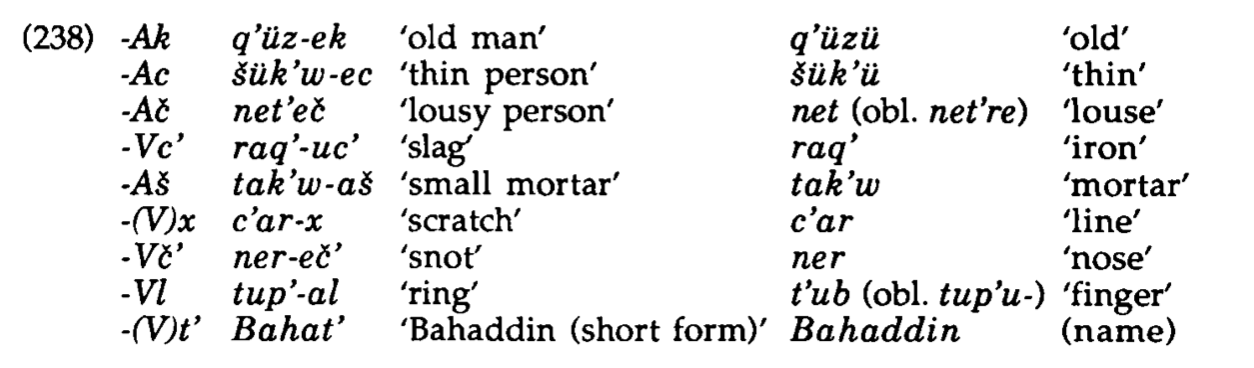
\includegraphics[width=.8\linewidth]{Lezgian/src/ex238.png}}
\end{figure}
\end{itemize}

\subsubsection{명사 복합}
\begin{itemize}
\item 레즈기어는 한정 복합이 존재하지 않는다. 즉, `N\textsubscript{1}의 N\textsubscript{2}'를 \textbf{N\textsubscript{1}N\textsubscript{2}}로 나타낼 수 없다.
\item N\textsubscript{1}과 N\textsubscript{2}가 쌍을 이루거나, 합쳐서 집단을 이루거나, 비슷한 의미를 가질 경우 둘을 연결하여 복합 명사를 만드는 경우는 존재한다.
\begin{figure}[H]
\centerline{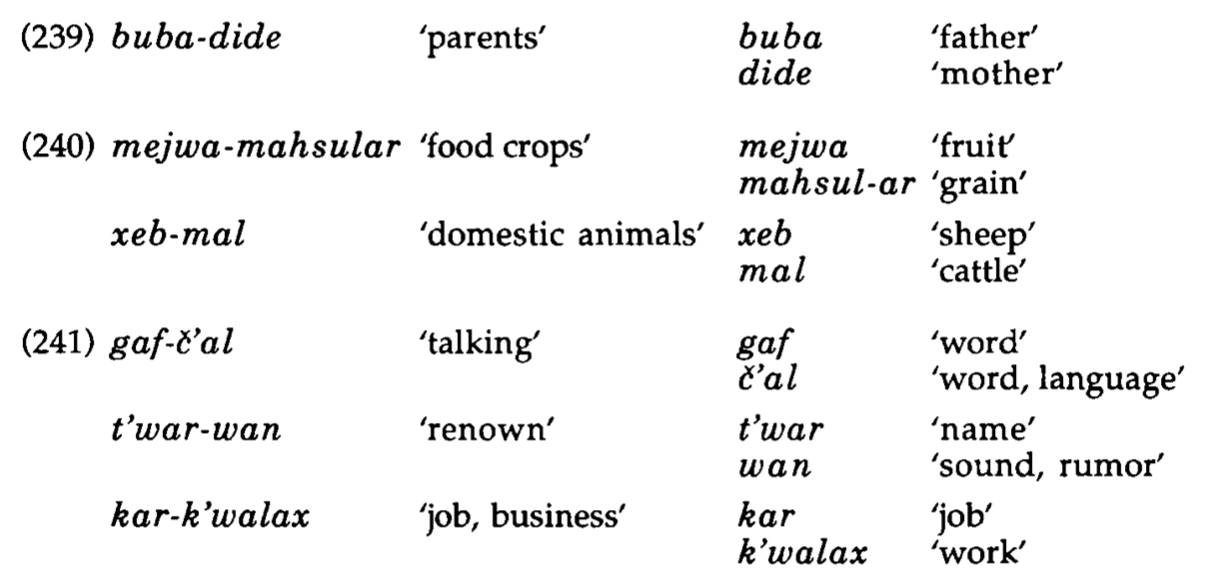
\includegraphics[width=.8\linewidth]{Lezgian/src/ex7-3-2.png}}
\end{figure}
\item 종종, 이 복합을 이루는 명사 중 하나는 독립적으로 나타날 수 없을 때도 있다. (크랜베리 형태소)
\begin{figure}[H]
\centerline{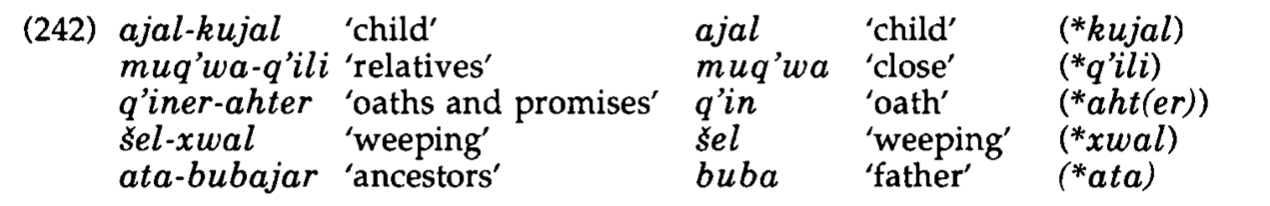
\includegraphics[width=.8\linewidth]{Lezgian/src/ex242.png}}
\end{figure}
\end{itemize}

\subsubsection{형용사로부터의 전환}
\begin{itemize}
\item 형용사는 실질화 형태소를 부착하여 명사로 파생시킬 수 있다. (8.1.1 참조)
\item 그러나 형태소 부착 없이 바로 형용사를 명사로 전환할 수도 있다. 이런 명사들은 다른 명사와 동일하게 굴절한다.
\item 이는 생산적인 과정이며, 주로 사람의 부정적인 성질을 나타내는 형용사에 많이 사용된다.
\begin{figure}[H]
\centerline{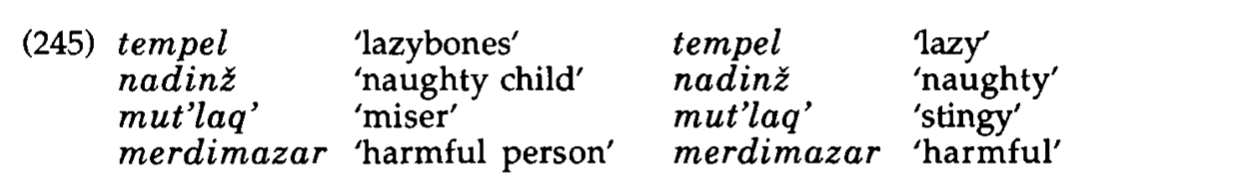
\includegraphics[width=.8\linewidth]{Lezgian/src/ex245.png}}
\end{figure}
\item 국적을 나타내는 형용사도 마찬가지.
\end{itemize}

\subsubsection{메아리 복합 명사}
\begin{itemize}
\item 해당 지역의 다른 언어들처럼 명사를 중첩하고 두 번째 단어의 어두 자음을 \textbf{m-}으로 교체하여 복합 명사를 만드는 과정이 존재한다. 
\item 그 결과 \textbf{N m-N'}의 의미는 `N and similar things' 이다.
\item 일반적으로 경멸적인 암시가 존재한다.
\begin{figure}[H]
\centerline{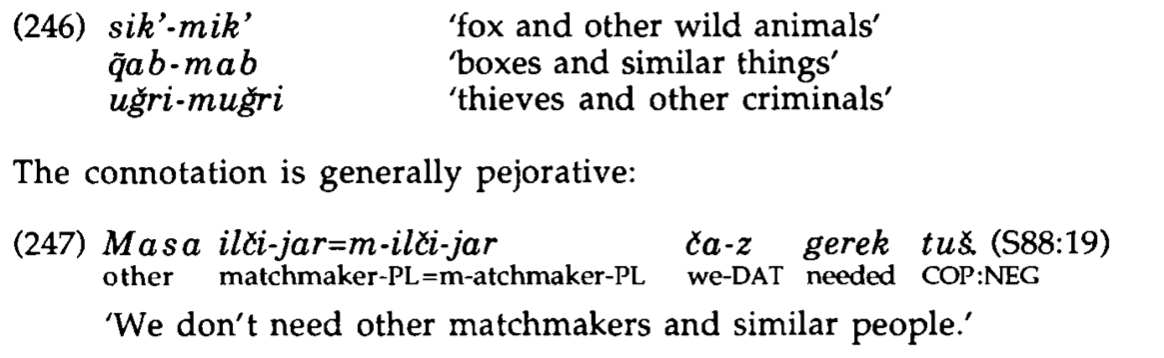
\includegraphics[width=.8\linewidth]{Lezgian/src/ex7-3-4.png}}
\end{figure}
\end{itemize}














